% Author: Till Tantau
% Source: The PGF/TikZ manual
\documentclass[tikz]{standalone}

\usepackage{tikz}
\usetikzlibrary{trees,snakes}
\begin{document}
\pagestyle{empty}
\tikzstyle{level 1}=[sibling angle=30, level distance=1cm]
\tikzstyle{level 2}=[sibling angle=20, level distance=.7cm]
\tikzstyle{level 3}=[sibling angle=10, level distance=.49cm]
\tikzstyle{every node}=[%fill,
		 				inner sep=0pt]
%\tikzstyle{edge from parent}=[snake=ticks,segment length=2mm,draw]
\tikzstyle{edge from parent}=[draw]


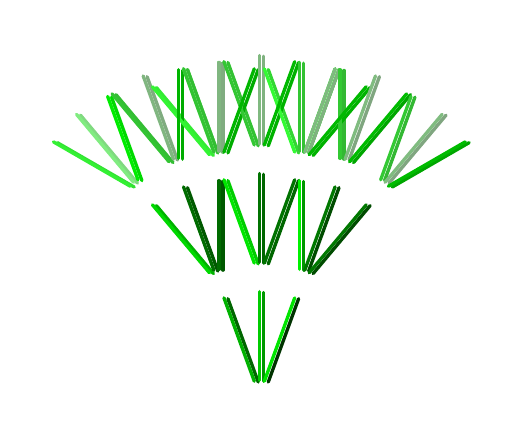
\begin{tikzpicture}
\begin{scope}[grow cyclic,shape=circle,very thick, cap=round, rotate=90] 
\node at (0,0) {} child [color=\A] foreach \A in {green!20!black,green!60!black,green!40!black}
    { node {} child [color=\A!50!\B] foreach \B in {green!50!black,green!50!black,green}
        { node {} child [color=\A!50!\B!50!\C] foreach \C in {green,white,green!80}
            { node {} }
        }
    };
\node at (0.01,0.05) {} child [color=\A] foreach \A in {green!90!black,green!80!black,green!70!black}
    { node {} child [color=\A!50!\B] foreach \B in {green!50!black,green!50!black,green}
        { node {} child [color=\A!50!\B!50!\C] foreach \C in {green,white,green!80}
            { node {} }
        }
    };
\end{scope}
\end{tikzpicture}

\end{document}